
%(BEGIN_QUESTION)
% Copyright 2011, Tony R. Kuphaldt, released under the Creative Commons Attribution License (v 1.0)
% This means you may do almost anything with this work of mine, so long as you give me proper credit

An operator claims that this flow-control system is not regulating process fluid flow at the correct rate.  Despite the fact that the PV reads equal to SP on the controller faceplate (both read 386 GPM in a 0-500 GPM range), the operator says he has reason to believe the actual flow rate is much lower than this (approximately 220 GPM) based on calculations of mass balance in a downstream process.  You happen to notice that the controller output reads 35\% on the faceplate:

$$\includegraphics[width=15.5cm]{i00362x01.eps}$$

Your first test is to measure loop current in the circuit connecting the flow transmitter to the flow controller.  There, your multimeter registers 11.05 milliamps.  Your next step is to record the pressure gauge's indication: 7 PSI.

\vskip 10pt

Identify the likelihood of each specified fault for this control system.  Consider each fault one at a time (i.e. no coincidental faults), determining whether or not each fault could independently account for {\it all} measurements and symptoms in this circuit.

% No blank lines allowed between lines of an \halign structure!
% I use comments (%) instead, so that TeX doesn't choke.

$$\vbox{\offinterlineskip
\halign{\strut
\vrule \quad\hfil # \ \hfil & 
\vrule \quad\hfil # \ \hfil & 
\vrule \quad\hfil # \ \hfil \vrule \cr
\noalign{\hrule}
%
% First row
{\bf Fault} & {\bf Possible} & {\bf Impossible} \cr
%
\noalign{\hrule}
%
% Another row
FT out of calibration (outputting wrong current) &  &  \cr
%
\noalign{\hrule}
%
% Another row
FIC input out of calibration (not interpreting signal properly) &  &  \cr
%
\noalign{\hrule}
%
% Another row
FIC output out of calibration (not sending correct mA signal to I/P) &  &  \cr
%
\noalign{\hrule}
%
% Another row
Pressure gauge out of calibration (not displaying pressure properly) &  &  \cr
%
\noalign{\hrule}
%
% Another row
I/P out of calibration (not outputting correct pressure) &  &  \cr
%
\noalign{\hrule}
%
% Another row
Control valve is oversized &  &  \cr
%
\noalign{\hrule}
%
% Another row
Control valve is undersized &  &  \cr
%
\noalign{\hrule}
%
% Another row
Control valve bench-set is improper &  &  \cr
%
\noalign{\hrule}
%
% Another row
FIC is poorly tuned &  &  \cr
%
\noalign{\hrule}
%
% Another row
Operator's mass-balance calculations are incorrect &  &  \cr
%
\noalign{\hrule}
} % End of \halign 
}$$ % End of \vbox

\underbar{file i00362}
%(END_QUESTION)





%(BEGIN_ANSWER)

% No blank lines allowed between lines of an \halign structure!
% I use comments (%) instead, so that TeX doesn't choke.

$$\vbox{\offinterlineskip
\halign{\strut
\vrule \quad\hfil # \ \hfil & 
\vrule \quad\hfil # \ \hfil & 
\vrule \quad\hfil # \ \hfil \vrule \cr
\noalign{\hrule}
%
% First row
{\bf Fault} & {\bf Possible} & {\bf Impossible} \cr
%
\noalign{\hrule}
%
% Another row
FT out of calibration (outputting wrong current) &  & $\surd$ \cr
%
\noalign{\hrule}
%
% Another row
FIC input out of calibration (not interpreting signal properly) & $\surd$ &  \cr
%
\noalign{\hrule}
%
% Another row
FIC output out of calibration (not sending correct mA signal to I/P) &  & $\surd$ \cr
%
\noalign{\hrule}
%
% Another row
Pressure gauge out of calibration (not displaying pressure properly) &  & $\surd$ \cr
%
\noalign{\hrule}
%
% Another row
I/P out of calibration (not outputting correct pressure) &  & $\surd$ \cr
%
\noalign{\hrule}
%
% Another row
Control valve is oversized &  & $\surd$ \cr
%
\noalign{\hrule}
%
% Another row
Control valve is undersized &  & $\surd$ \cr
%
\noalign{\hrule}
%
% Another row
Control valve bench-set is improper &  & $\surd$ \cr
%
\noalign{\hrule}
%
% Another row
FIC is poorly tuned &  & $\surd$ \cr
%
\noalign{\hrule}
%
% Another row
Operator's mass-balance calculations are incorrect &  & $\surd$ \cr
%
\noalign{\hrule}
} % End of \halign 
}$$ % End of \vbox

%(END_ANSWER)





%(BEGIN_NOTES)

{\bf This question is intended for exams only and not worksheets!}.

%(END_NOTES)


